\section{Model and inferential targets}
\label{sec:model}

\subsection{A branching experiment with a known observation scale}
\label{sec:model-branching}

Consider one generation of transmission with $n\ge1$ primary infections. Conditional on the reproduction number $R_t>0$, the offspring counts of primary cases are independent negative binomial variables \citep{lloydsmith2005superspreading}:
\begin{equation}
  X_{i,t}\mid R_t\sim\NB(k,\,k/(k+R_t)),\qquad
  \E(X_{i,t}\mid R_t)=R_t,\quad
  \Var(X_{i,t}\mid R_t)=R_t+\frac{R_t^2}{k},
  \label{eq:offspring}
\end{equation}
where $k>0$ controls individual heterogeneity. Each secondary infection is independently reported with probability $\rho\in(0,1]$. Summation and binomial thinning give
\begin{equation}
  C_t\mid n,R_t\sim\NB(nk,\,k/(k+\rho R_t)),\qquad
  \E(C_t\mid n,R_t)=\rho nR_t,\qquad
  \Var(C_t\mid n,R_t)=\rho nR_t+\frac{\rho^2nR_t^2}{k}.
  \label{eq:observed}
\end{equation}
Define $m=\rho n$ and $\Rhat_t=C_t/m$. The scale $m$ is the expected reported count at $R_t=1$, not the realised count $C_t$.

The baseline assumptions are fixed, known $\rho$ with independent reporting (H1); conditionally independent offspring as in Eq.~\eqref{eq:offspring} (H2); fixed, known $k$ (H3); and a fixed or exogenous $n$ that does not depend on transmission (H4). Write $\E(R_t)=\Rbar>0$ and $\Var(R_t)=v_R<\infty$. Across periods, counts are independent given the whole transmission trajectory, each with conditional law~\eqref{eq:observed}. These are repeated branching experiments; they do not assert that naturally evolving incidence is exogenous. Dividing by an assumed $\rho_0\ne\rho$ gives conditional mean $(\rho/\rho_0)R_t$, a multiplicative bias that more cases do not remove.

The conditional counting variance combines offspring randomness and omission. Conditioning on the total number of secondary infections splits it into $(R_t+R_t^2/k)/n$ and $(1-\rho)R_t/(\rho n)$. The term linear in $R_t$ is therefore not purely reporting noise; it remains under complete reporting.

\subsection{Current values, realised means and process means}
\label{sec:model-targets}

For the current target, $\E(\Rhat_t\mid R_t)=R_t$ and $\Var(\Rhat_t\mid R_t)=(R_t+\rho R_t^2/k)/m$, which attains the Cram\'er--Rao bound for estimators unbiased for every $R_t$ under this likelihood (Appendix~\ref{app:model}).

\begin{proposition}[One period, two targets]
\label{prop:average}
Under H1--H4, let $A=\Rbar+\rho(\Rbar^2+v_R)/k$. Then
\begin{equation}
  \E[(\Rhat_t-R_t)^2]=\frac{A}{m},\qquad
  V(m):=\E[(\Rhat_t-\Rbar)^2]=v_R+\frac{A}{m}.
  \label{eq:var-average}
\end{equation}
Among estimators based on this period's count that are conditionally unbiased for $R_t$, $\Rhat_t$ minimises both risks.
\end{proposition}

The proof (Appendix~\ref{app:prop1}) squares
\begin{equation}
  \Rhat_t-\Rbar=(\Rhat_t-R_t)+(R_t-\Rbar),
  \label{eq:error-split}
\end{equation}
whose two terms are uncorrelated. Between-period transmission variation is part of the signal for the current value and sampling error for the process mean, which is a mean under a stated stationary law and not automatically a seasonal average of a nonstationary epidemic.

For $v_R>0$ define the crossover scale $\mx=A/v_R$, the expected count at which the two terms of $V(m)$ are equal. Its meaning is the one it has in small-area estimation \citep{fay1979estimates}. The best linear predictor of $R_t$ from $\Rhat_t$ under the stated moments is
\begin{equation}
  \Rbar+\gamma(m)(\Rhat_t-\Rbar),\qquad
  \gamma(m)=\frac{v_R}{v_R+A/m}=\frac{m}{m+\mx},
  \label{eq:shrink-weight}
\end{equation}
so $\mx$ is the count at which shrinkage gives the direct estimate half its weight. Doubling $m$ through $n$ at fixed $\rho$, $k$ and transmission law reduces process-mean risk by the fraction $1/[2(1+m/\mx)]$: one quarter at $m=\mx$, and less beyond it. Changing $\rho$ changes $A$ as well as $m$. The scale $\mx$ describes the selected estimator and target; it does not mark a point where information stops accumulating.

\begin{corollary}[A fixed set of observed periods]
\label{cor:targets}
Under H1--H4 and conditional independence of counts given $R_{1:T}$, let $\Rbar_T$ denote the mean of $R_1,\dots,R_T$ and $\overline{\Rhat}_T$ the mean of $\Rhat_1,\dots,\Rhat_T$. If the $R_t$ share common marginal moments, the two mean targets have risks:
\begin{equation}
  \E[(\overline{\Rhat}_T-\Rbar_T)^2]=\frac{A}{Tm},\qquad
  \E[(\overline{\Rhat}_T-\Rbar)^2]=B_T+\frac{A}{Tm},
  \qquad B_T=\Var(\Rbar_T).
  \label{eq:target-means}
\end{equation}
In Eq.~\eqref{eq:target-means}, $B_T=v_R/T$ for independent, identically distributed $R_t$. For a stationary process with $\Cov(R_t,R_{t+h})=v_R\phi^{|h|}$, $|\phi|<1$, $B_T=v_RS(\phi,T)/T^2$ exactly, with
\begin{equation}
  S(\phi,T)=T+2\sum\nolimits_{h=1}^{T-1}(T-h)\phi^h
  =\frac{T(1+\phi)}{1-\phi}-\frac{2\phi(1-\phi^T)}{(1-\phi)^2}.
  \label{eq:ar-sum}
\end{equation}
\end{corollary}

The realised-mean identity needs only conditionally independent counting errors, not independent transmission levels. More cases in the same periods remove its counting error, while process-mean risk tends to $B_T$; only more periods reduce $B_T$, at a rate set by their dependence. Positive persistence reduces the gain from adjacent periods. Spatial averaging behaves analogously: for $J$ units with transmission variance $v_R$ and mean pairwise correlation $\bar c$, the averaged transmission level has variance:
\begin{equation}
  \Var(J^{-1}{\textstyle\sum_{j=1}^J}R_{j,t})=v_R[\bar c+(1-\bar c)/J].
  \label{eq:pooling}
\end{equation}
Figure~\ref{fig:targets} plots these risks, with known-truth Monte Carlo checks, and Table~\ref{tab:targets} collects them.

\subsection{An observed denominator}
\label{sec:model-observed}

Surveillance ratios divide by an observed count rather than by a known scale. Let the denominator be the reported count of the primary generation, $M_t\sim\Bin(n,\rho)$, independent of the offspring given $n$, and let $\tilde R_t=C_t/M_t$. Because $M_t=m(1+u_t)$ with $\Var(u_t)=(1-\rho)/m$, a delta expansion (Appendix~\ref{app:observed-denominator}) gives
\begin{equation}
  \E[(\tilde R_t-R_t)^2]\approx\frac{A+(1-\rho)(\Rbar^2+v_R)}{m},
  \label{eq:observed-denominator}
\end{equation}
so the crossover scale moves to $\mx+(1-\rho)(\Rbar^2+v_R)/v_R$. With $\Rbar=1.15$, $v_R=0.04$, $k=0.35$ and $\rho=0.25$ ($A=2.1232$) it rises from 53.1 to 78.6. Monte Carlo with 400,000 draws per scale (Table~\ref{tab:ma_targets_observed}) puts the observed-denominator error at 1.59, 1.51 and 1.49 times $A/m$ for $m=50$, 200 and 1000, close to the delta value of 1.48. At $m=10$ the ratio is 2.42 and the delta form understates the error, because small denominators inflate the ratio.

\begin{table}[!tbp]
\centering
\small
\setlength{\tabcolsep}{4pt}
\caption{Inferential targets and exact mean squared errors. The fixed-reporting column assumes H1--H4; the volatile-reporting column assumes H2--H5 and, for averages, independent reporting probabilities independent of the transmission path. Counting errors are conditionally independent across periods. $B_T=\Var(\Rbar_T)$ equals $v_R/T$ for independent, identically distributed transmission and $v_RS(\phi,T)/T^2$ under the stated stationary autocovariance. With the previous observed count as denominator, the current-value entry under fixed reporting becomes approximately $[A+(1-\rho)(\Rbar^2+v_R)]/m$ (Eq.~\ref{eq:observed-denominator}; Table~\ref{tab:ma_targets_observed}).}
\label{tab:targets}
\begin{tabularx}{\linewidth}{>{\raggedright\arraybackslash}X>{\centering\arraybackslash}p{0.13\linewidth}>{\centering\arraybackslash}p{0.24\linewidth}>{\centering\arraybackslash}p{0.27\linewidth}}
\toprule
Target & Estimator & Fixed, known reporting & Unobserved volatile reporting \\
\midrule
Current $R_t$ & $\Rhat_t$ & $A/m$ & $v_H+A_H/m$ \\
Realised mean $\Rbar_T$ & $\overline{\Rhat}_T$ & $A/(Tm)$ & $(v_H+A_H/m)/T$ \\
Process mean $\Rbar$ & $\overline{\Rhat}_T$ & $B_T+A/(Tm)$ & $B_T+(v_H+A_H/m)/T$ \\
\bottomrule
\end{tabularx}
\end{table}


\begingroup\scriptsize\setlength{\tabcolsep}{2pt}
\begin{longtable}{@{}>{\raggedright\arraybackslash}p{\dimexpr 0.2400\linewidth-3.500pt\relax}>{\raggedright\arraybackslash}p{\dimexpr 0.1000\linewidth-3.500pt\relax}>{\raggedright\arraybackslash}p{\dimexpr 0.1000\linewidth-3.500pt\relax}>{\raggedright\arraybackslash}p{\dimexpr 0.1000\linewidth-3.500pt\relax}>{\raggedright\arraybackslash}p{\dimexpr 0.1000\linewidth-3.500pt\relax}>{\raggedright\arraybackslash}p{\dimexpr 0.1000\linewidth-3.500pt\relax}>{\raggedright\arraybackslash}p{\dimexpr 0.1000\linewidth-3.500pt\relax}>{\raggedright\arraybackslash}p{\dimexpr 0.1000\linewidth-3.500pt\relax}@{}}
\caption{Point-target error with a known versus an observed denominator}\label{tab:ma_targets_observed}\\
\toprule
m & Known denominator A/m & MC (SE) & Observed denominator (A + (1 - rho)(Rbar\textasciicircum{}2 + v\_\allowbreak{}R))/m & MC (SE) & MC observed / A/m & Zero denominators & +0.5 variant MC (SE) \\
\midrule
\endfirsthead
\multicolumn{8}{@{}l}{\textit{(continued)}}\\
\toprule
m & Known denominator A/m & MC (SE) & Observed denominator (A + (1 - rho)(Rbar\textasciicircum{}2 + v\_\allowbreak{}R))/m & MC (SE) & MC observed / A/m & Zero denominators & +0.5 variant MC (SE) \\
\midrule
\endhead
\midrule
\multicolumn{8}{r@{}}{\textit{(continued on next page)}}\\
\endfoot
\bottomrule
\endlastfoot
10 & 0.21232 & 0.21304 (0.00055) & 0.31451 & 0.51453 (0.00482) & 2.423 & 0 & 0.42529 (0.00276) \\
50 & 0.04246 & 0.04234 (0.00010) & 0.06290 & 0.06745 (0.00019) & 1.588 & 0 & 0.06589 (0.00018) \\
200 & 0.01062 & 0.01060 (0.00002) & 0.01573 & 0.01601 (0.00004) & 1.508 & 0 & 0.01592 (0.00004) \\
1000 & 0.00212 & 0.00212 (0.00000) & 0.00315 & 0.00316 (0.00001) & 1.489 & 0 & 0.00316 (0.00001) \\
\end{longtable}
\vspace{-.5\baselineskip}
\noindent\begin{minipage}{\linewidth}\footnotesize\raggedright
Parameters Rbar = 1.15, v\_\allowbreak{}R = 0.04, k = 0.35, rho = 0.25 (A = 2.1232); 400,000 Monte Carlo draws per m. Crossing scale m\_\allowbreak{}x = A/v\_\allowbreak{}R = 53.08 with a known denominator and (A + (1 - rho)(Rbar\textasciicircum{}2 + v\_\allowbreak{}R))/v\_\allowbreak{}R = 78.63 when the denominator is the observed previous count (delta approximation). At m = 10 the delta approximation understates the Monte Carlo error of the observed-denominator estimator. Zero denominators: draws with a zero previous count are excluded from the ratio estimator (share shown); the +0.5 variant (C\_\allowbreak{}t + 0.5)/(C\_\allowbreak{}prev + 0.5) keeps every draw.
\end{minipage}\par
\endgroup


\begin{figure}[!tbp]
\centering
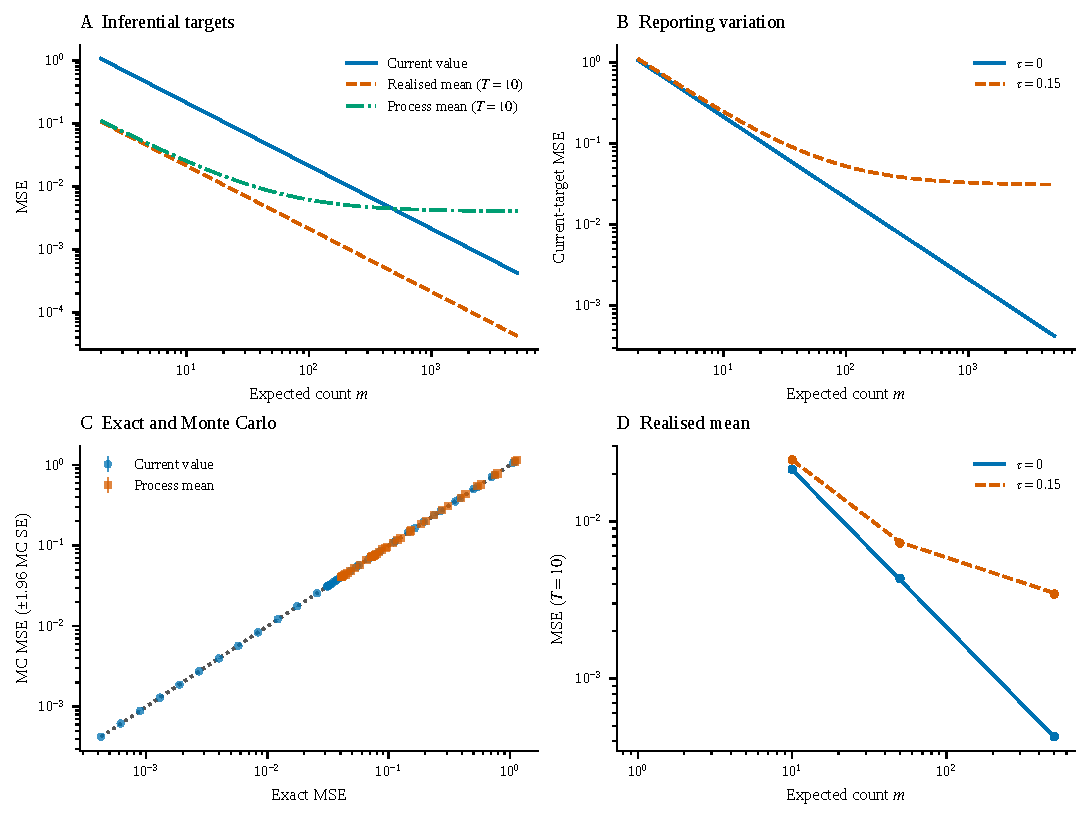
\includegraphics[width=0.92\linewidth]{figures/fig_01_targets.pdf}
\caption{Model risks for the three targets. (A) Mean squared error against expected count $m$ for the current value, the realised mean and the process mean over $T=10$ independent periods. (B) Current-value risk with fixed reporting ($\tau=0$) and with period-level reporting variation ($\tau=0.15$). (C) Exact risks against known-truth Monte Carlo estimates with 1.96 Monte Carlo standard errors. (D) Realised-mean risk over $T=10$ periods at three scales. Parameters: $\Rbar=1.15$, $v_R=0.04$, $k=0.35$, $\rho=0.25$. Counts are simulated under the fixed-exposure model, so the curves describe that model and not the hospital data.}
\label{fig:targets}
\end{figure}
